% 固定来源PDF印刷页50第23题正三棱柱图的矢量示意重绘。
% 仅表示顶点、棱和题目指定线段；投影不按比例，不据图添加度量条件。
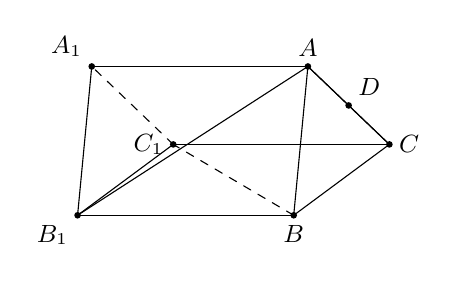
\begin{tikzpicture}[x=.9cm,y=.9cm,line cap=round,line join=round,font=\small]
  \coordinate (Aone) at (0,2.25);
  \coordinate (Bone) at (-.2,.15);
  \coordinate (Cone) at (1.15,1.15);
  \coordinate (A) at (3.05,2.25);
  \coordinate (B) at (2.85,.15);
  \coordinate (C) at (4.2,1.15);
  \coordinate (D) at (3.625,1.7);

  % Prism edges. The hidden far-base edge is dashed in this view.
  \draw (Aone)--(Bone)--(Cone);
  \draw[dashed] (Cone)--(Aone);
  \draw (A)--(B)--(C)--cycle;
  \draw (Aone)--(A) (Bone)--(B) (Cone)--(C);
  % Mark the source-defined midpoint D on AC and the lines used in the question.
  \draw (A)--(D)--(C);
  \draw (Bone)--(A);
  \draw[dashed] (B)--(Cone);
  \fill (Aone) circle (1.2pt) (Bone) circle (1.2pt) (Cone) circle (1.2pt)
        (A) circle (1.2pt) (B) circle (1.2pt) (C) circle (1.2pt) (D) circle (1.2pt);
  \node[above left] at (Aone) {$A_1$};
  \node[below left] at (Bone) {$B_1$};
  \node[left] at (Cone) {$C_1$};
  \node[above] at (A) {$A$};
  \node[below] at (B) {$B$};
  \node[right] at (C) {$C$};
  \node[above right] at (D) {$D$};
\end{tikzpicture}
